% テーブルの太線代替(未定義エラー回避)
\newcommand{\thline}{\hline}

\subsubsection{概要}
きなこチームでは,
自己位置推定にemcl2\_ros2を,
ナビゲーションには自作したkinako\_nav\cite{kinako_nav_github}を採用した.
圧縮した3次元地図の利用と自己位置推定の信頼性向上を目的に,
emcl2\_ros2を拡張した.
具体的には,
圧縮地図の読み出し機能を追加し,
もともと2次元スキャンのみ対応していたemcl2\_ros2を3次元点群に対応させた.
ただし,
3次元の自己位置推定は計算量が大きいため,
自由度は2次元(x, y, yaw)に制限した.
また,
3D LiDARの点群から高さ領域を指定して抽出し,
走行中に使用する高さを切り替える機能を実装した.
これにより,
人が多い場所では地上から離れた高さの点群を使うなど,
場所ごとに特徴的な高さの点群を使い分けられる.

本チームでは, 
当初, navigation2を採用していたが, 
つくばチャレンジのような動的障害物や対向ロボットが頻繁に交錯する実環境において, 以下の課題に直面した. 
\begin{itemize}
\item 複雑なスタック構成により処理が重くなり, リアルタイムな軌道更新が困難
\item 多数のプラグインとパラメータの相互依存により, 環境に対する最適なチューニングが困難
\item ローカルプランナーの計算窓の制約上, 他のロボットに相当接近してからでなければ回避行動を開始できず衝突のリスクが残存
\item グローバルプランナー, ローカルプランナー, およびリカバリ動作の切り替えロジックが複雑であり, 状況に応じたスムーズなモード遷移が困難
\end{itemize}

これらの課題を根本から解決するため, 
Fast Marching Method (FMM) を用いたナビゲーションシステムを開発した. 
本システムは, 
LiDARの観測範囲全域を単一のポテンシャル場として計算するため, 
経路計画と障害物回避を単一の処理系で完結させることが可能となった. 


FMMの計算量は O(NlogN) と極めて効率的であるため, 
LiDARが捉えた観測範囲全域の情報をリアルタイムにポテンシャル場へ反映できる. 
これにより, 遠方の対向ロボットや障害物を早い段階で検知し, 
余裕を持った予見的な回避行動が可能となった. 

空間の全座標においてゴールへ向かう勾配が定義されているため, 
不測の回避行動によって本来の予定進路から外れた場合でも, 
瞬時に現在地からの最適ルートを指し示すことができる. 
この特性により, 混雑環境下においても極めて堅牢な自律走行を達成した. 
% さらに,
% DWBやMPCといったローカルプランナーは候補パスのみを評価している.
% つくばチャレンジのように,
% どこからでもロボットや人が接近する状況では,
% LiDARの計測範囲全体の情報を経路計画に用いたい.


\subsubsection{占有格子地図の圧縮}
まず, 占有格子地図の圧縮を行った.
つくばチャレンジの地図は表\ref{tab:vq_compression_result}に示すように非常に大きい容量を持つ.
地図はGLIM\cite{glim}\cite{glim_github}を用いて3次元で作成し,
点群地図を占有格子地図に変換してから圧縮した.
圧縮にはvq\_occupancy\_compressor\cite{vq_occupancy_compressor_github}を使用した.

\begin{table}[tb]
  \centering
	\caption{Size of VQ map}
  \label{tab:vq_compression_result}
  \small
	\begin{tabular}{lc}
		\\
    \thline
		地図容量 & 30.9GB \\
    \hline
		実環境における規模 & 795.2$\times$523.6$\times$74.2m \\
    \hline
    解像度    & 0.1m/voxel \\
    \thline
  \end{tabular}
\end{table}

圧縮した結果, \ref{tab:compression_result}に示すように,
地図容量は74.6MBとなり, 圧縮率は0.0024となった.
\begin{table}[tb]
  \centering
	\caption{compression result}
  \label{tab:compression_result}
  \small
	\begin{tabular}{lc}
		\\
    \thline
		圧縮地図の容量 & 74.6MB \\
    \hline
		圧縮率 & 0.0024 \\
    \thline
  \end{tabular}
\end{table}


\subsubsection{開発したナビゲーションシステム}
システムの開発のために以下のいくつかのパッケージを作成した.

\begin{itemize}
  \item imu\_rpy\_pose: IMU角速度を積分し, 位置・姿勢を算出
  \item obstacle\_tracker: スキャンをクラスタリングして障害物マスクを生成
  \item pointcloud2\_cutter: ロボットの位置によって自己位置推定に最適な点群を高さ領域で切り出し. ロボットの全高領域はスキャンを生成
  \item waypoint\_manager: ウェイポイントの管理
  \item vector\_field\_planner: ベクトル場でローカル速度指令を生成するプランナ
  \item velocity\_smoother: 速度指令を平滑化
\end{itemize}

\subsubsection{システム統合}
きなこチームのシステム構成を図\ref{fig:kinako_system}, 図\ref{fig:kinako_nav}に示す.
\begin{figure}[h]
  \begin{center}
    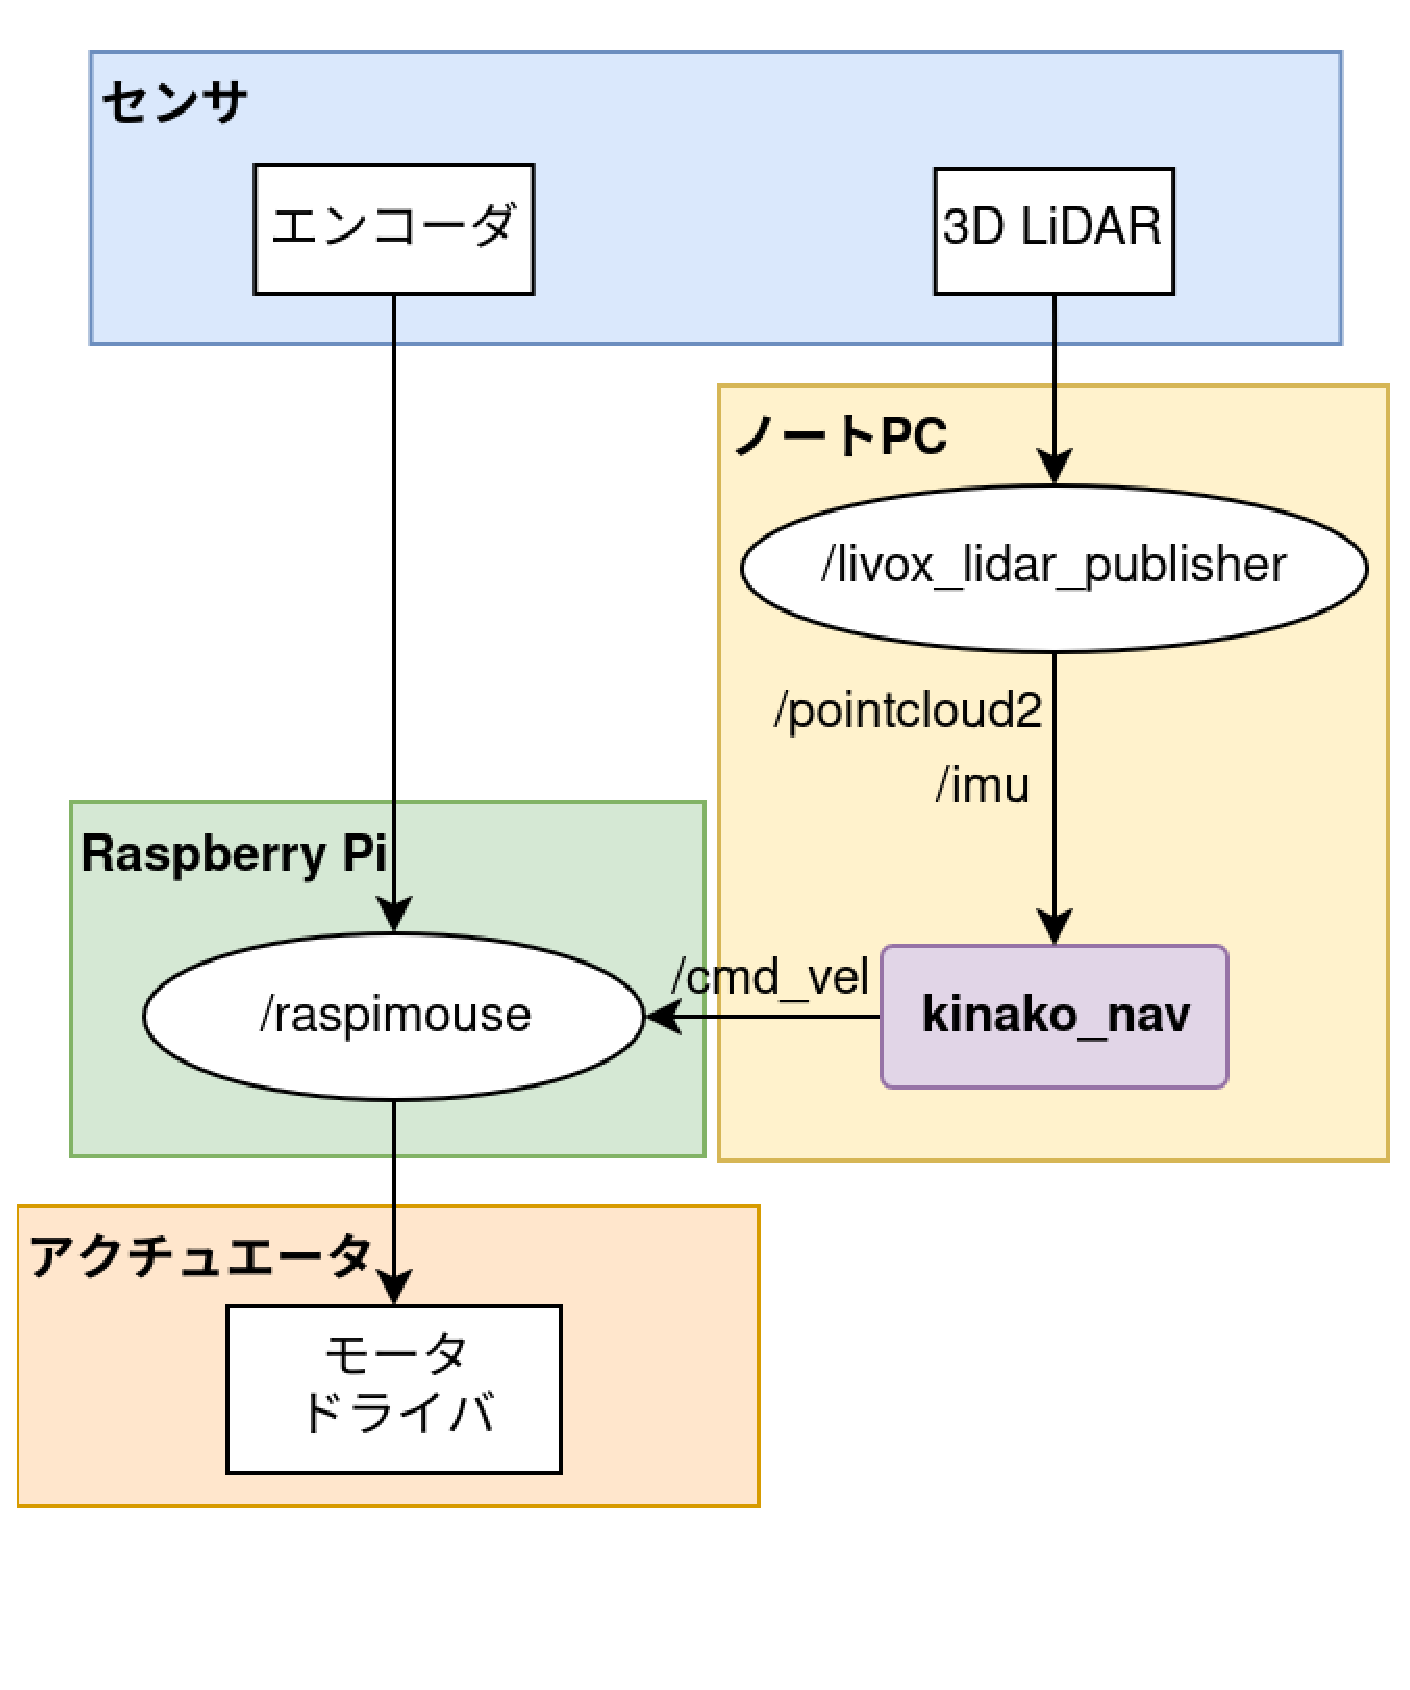
\includegraphics[width=1.0\linewidth]{figs/kinako_system.eps}
    \caption{きなこチームのシステム構成}
    \label{fig:kinako_system}
  \end{center}
\end{figure}

\begin{figure}[h]
  \begin{center}
    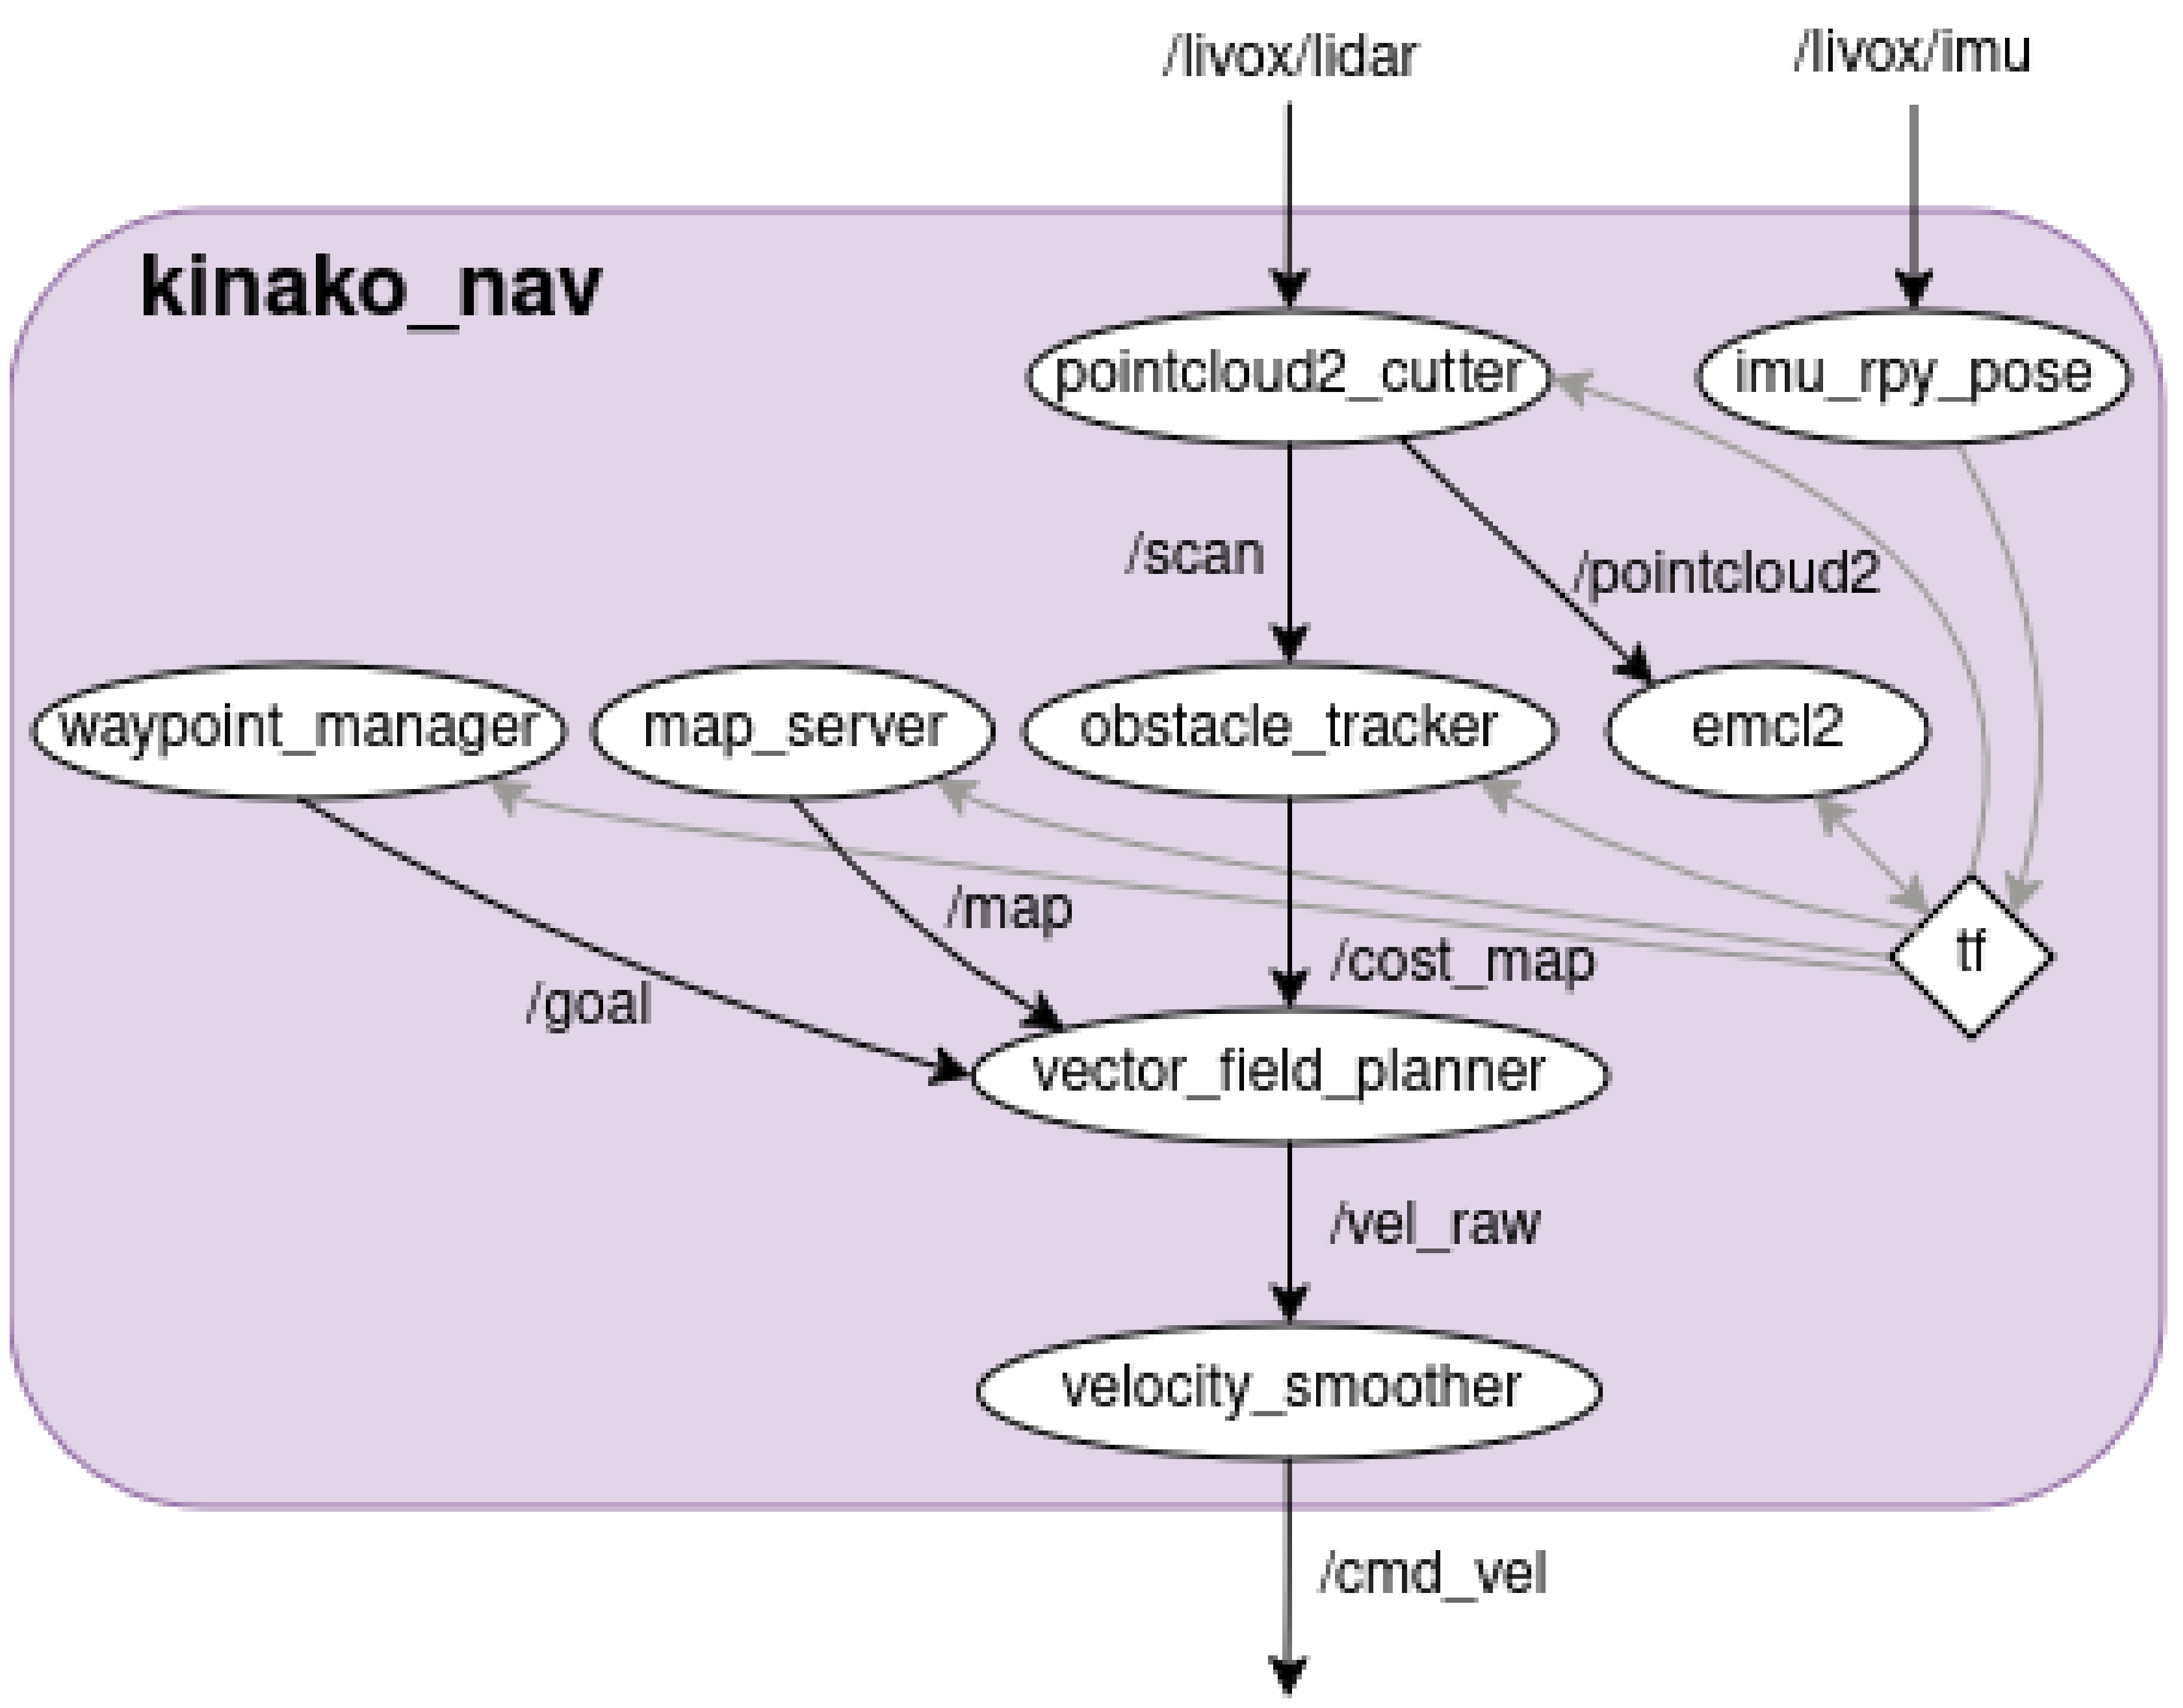
\includegraphics[width=1.0\linewidth]{figs/kinako_nav.eps}
    \caption{kinako\_navのシステム構成}
    \label{fig:kinako_nav}
  \end{center}
\end{figure}